\subsubsection{An independent coastal wind reference}
\label{sec:independent-coastal-wind}

For the Channel Coast, an independent wind climatology provides the corresponding
orientation reference. ERA5 hourly reanalysis \cite{era5_hourly}, retrieved through
the Open-Meteo Historical Weather API \cite{open_meteo_historical}, supplies wind
speed and direction at 10 and \SI{100}{\metre} above ground. The reference covers
ten complete years, 2016--2025. It uses nine representative cells: the nearest
ERA5 cells to the centres of a regular $3\times3$ partition of the existing
Channel Coast box. Model selection is explicitly ERA5, on its $0.25^\circ$ grid,
with neither a land-cell preference nor elevation downscaling. This sparse
regional sample is adequate for an indicative orientation comparison; it does
not resolve local coastal lift or reproduce weather along individual flights.

If $s$ is wind speed and $\phi$ the meteorological direction, measured clockwise
from north and indicating where the wind comes from, the east and north
components of air motion are
\begin{equation}
 u=-s\sin\phi,\qquad v=-s\cos\phi,\qquad
 \theta_w=\operatorname{atan2}(\langle v\rangle,\langle u\rangle).
 \label{eq:regional-wind-axis}
\end{equation}
The averages include every archived hour and weight cells by
$\cos(\mathrm{latitude})$ to approximate represented area. Direction angles
are never averaged arithmetically. The resulting \emph{towards} angle is
counterclockwise from east, then reduced modulo $180^\circ$ for comparison
with the undirected PCA axis. Thus a meteorological wind \emph{from}
\SI{\StatWindSurfaceFrom}{\degree} corresponds to the reference axis
\SI{\StatWindSurfaceAngle}{\degree} used here.

\begin{figure}[htbp]
 \centering
 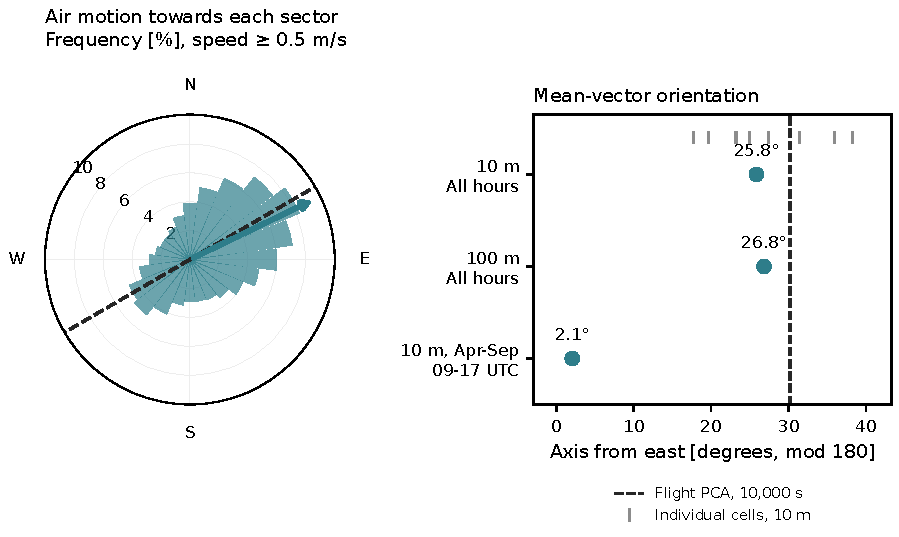
\includegraphics[width=\linewidth]{generated/ch3_channel_wind}
 \caption{ERA5 coastal wind reference and the paraglider covariance axis at
 \SI{10000}{\second}. Left: weighted frequency of air motion \emph{towards}
 15-degree sectors at \SI{10}{\metre}, excluding speeds below
 \SI{0.5}{\metre\per\second} and normalising the retained observations.
 The coloured arrow is the mean wind vector direction, calculated using all
 hours; the dashed line is the undirected flight axis. Right: mean-vector
 axes for the annual \SI{10}{\metre} reference, an annual \SI{100}{\metre}
 check, and a \SI{10}{\metre} April--September, 09--17 UTC check.
 Grey marks show the nine separate annual cell means, not confidence limits.
 The same \num{\StatWindFlights} coastal flights define the PCA reference
 in all three comparisons.}
 \label{fig:independent-coastal-wind}
\end{figure}

The annual surface-wind axis, \SI{\StatWindSurfaceAngle}{\degree}, is close to
the flight axis, \SI{\StatWindFlightAngle}{\degree}: their separation is
\SI{\StatWindSurfaceDifference}{\degree}. The \SI{100}{\metre} annual axis,
\SI{\StatWindHundredAngle}{\degree}, gives a similar separation of
\SI{\StatWindHundredDifference}{\degree}. However, selecting April--September
and 09--17 UTC inclusive rotates the surface reference to
\SI{\StatWindWarmDayAngle}{\degree}, increasing the separation to
\SI{\StatWindWarmDayDifference}{\degree}. Annual alignment therefore does
not persist under this simple seasonal and daytime selection. This window
is an operational sensitivity check, not an estimate of actual flight times.

The main ratio $\|\langle\mathbf w\rangle\|/\langle\|\mathbf w\|\rangle$
is only \num{\StatWindSurfaceResultant}: substantial directional cancellation
occurs across the observed winds. This ratio measures neither confidence in
the angle nor the fraction of winds in its sector. More fundamentally, a mean
wind vector and a centred displacement covariance are different statistics.
A common constant additive wind shifts displacement by $\tau\mathbf w$ and
is removed by centring at fixed lag. Variable winds between flights or within
tracks, and route choices responding to them, can still orient the covariance;
climatological alignment alone cannot establish those mechanisms.

All nine hourly API responses are archived without loss, with coordinates,
request URLs, units, retrieval times and SHA-256 identities. The compressed
inputs occupy about \SI{6.3}{\mega\byte}; they can be reused offline. Taking one
value every six hours, for every possible UTC starting phase, changes the
annual axis by at most $0.52^\circ$. Hourly resolution is retained because its
storage cost is small and it preserves the wind distribution and flexible
time-of-day checks. The ten-year reference reduces dependence on a single year,
but it is not matched to the full flight archive, take-off conditions or flight
altitudes. The evidence supports an indicative annual orientational association,
with clear temporal sensitivity, rather than a causal explanation of the
coastal ellipse or of differences between equipment groups.
